\chapter[Task 01]{\#01: Ising Model}

\resp{David Weingut}

\section{Theoretical Basis}
 The Ising model is a simplified version of the spin-spin interaction on a lattice. The spins are assumed to be $\pm1$ and interactions are only allowed between direct neighbours.
 
 This is achieved by the following Hamiltonian, equation \ref{eq:isinghamilton}, where $J_{ij}$ is the coupling strength between vertices $i$ and $j$ and $s_i$ is the spin value of Vertex $i$. $M$ is the external magnetic field. The sum touches each interacting pair once.
 
 \begin{equation}
 	\mathcal{H} = -\sum_{i<j} J_{ij} s_i s_j - \sum_{i} M s_i \label{eq:isinghamilton}
 \end{equation}

In most cases the external magnetic field is set to zero, which eliminates the latter part and leaves only the interaction term. The sum over spin pairs can also be expressed as a sum over the edges.

For a two dimensional grid the behaviour has been solved analytically in 1944 by Onsager\cite{Onsager}. For an arbitrary structured complex network there hasn't been any due to the the enormous number of configurations.

\section{Simulation}
For the simulating approach simulated annealing was chosen to get the time evolution for the Ising model. A single flip Metropolis sampler was chosen due to its good performance and ease of implementation.

To find the critical temperature $T_c$ I found the magnetization $M$ to be most consistent.
This is due to it being a monotonous function of temperature which makes it very easy to find the temperature where it crosses a certain threshold.
The magnetical susceptibility $\chi$ was regarded as promising in the beginning because it is supposed to peak at $T=T_c$ but its volatile nature with very large uncertainties near the peak made finding the critical temperature a very unreliable task with strong fluctuations.
The heat capacity $C_v$ was very similar, supposed to peak at $T_c$ but rather unreliable in helping find it.
Additionally for the network families I tested, $\chi$ and $C_v$ peaked at different temperatures, with no way to discern reliably which of the peaks was the more reliable for my research, the representative behaviour is shown in the appendix, figure \ref{fig:cv-chi-01}.

The theoretical predictions of the model's behaviour are manifold.
I tried to match the results of my simulations to the research paper of Leone et al.\cite{Leone2002}.
They provide a theoretical result for the critical temperature as a function of the first and second moments of the degree distribution.
A problem I encountered with this equation is that I couldn't match the behaviour shown in the paper, neither via a replication of the formula nor via my simulation results.
The most obvious is the missing divergence of the critical temperature for degree exponents below 3.
In figure \ref{fig:EM-SF-2.0-01} I show the dependence of magnetization and energy vs temperature.

\section{Results for Random Graphs}
In the following the behaviour of the critical temperature, determined as above, is explored for some families of random graphs. As the behaviour should not depend on the size of the graph in a strong way, for ER and WS graphs the size is chosen to be 500 nodes, while for the SBM the size is chosen to 
\subsubsection{Erdös-Renyi}
For the Erdös-Renyi graphs the behaviour vs the mean degree is studied.
\begin{figure}[h]
	\centering
	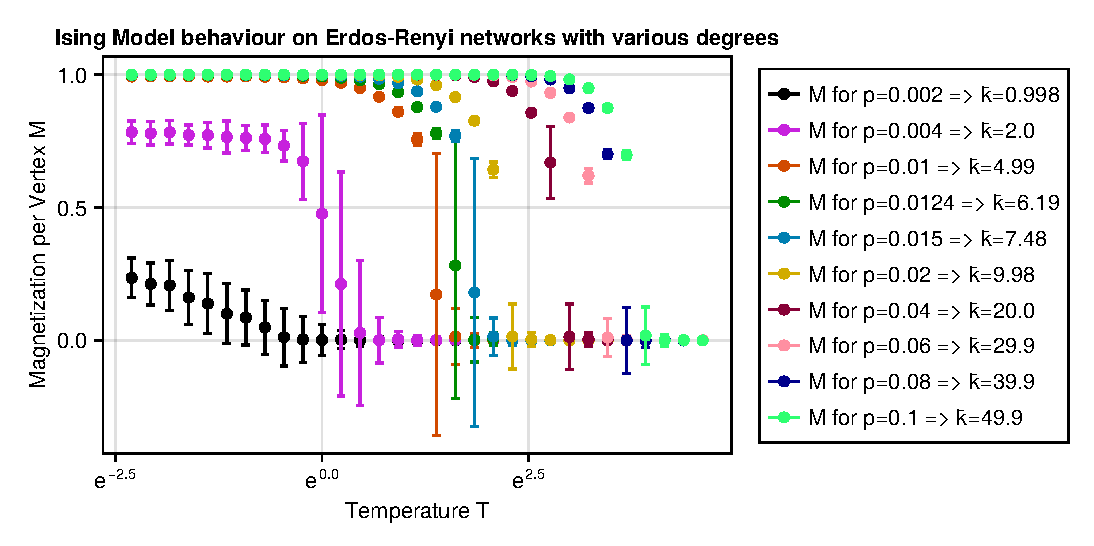
\includegraphics{Ising_magnetization_ER_many}
	\caption{Behaviour of the magnetization of an Ising model on-top an Erdös-Renyi graph for a collection of temperatures and mean degrees}
	\label{fig:M-ER-0.1}
\end{figure}
One can see that the magnetization for a fixed temperature strongly depends on the average degree.
This can be explained intuitively as for the lower degrees there are lot of independent components in the networks who don't interact with each other but by this lower the total average magnetization.
The high degree networks in contrast have a structure which makes it very hard for individual spins who are surrounded by parallel peers to flip due to the energy change based flipping probabilities.


\subsubsection{Watts-Strogatz}
For the Watts-Strogatz small world graphs the dependence on the rewiring probability is looked into. For low ones the onset temperature rises with the probability but stagnates for around $p=0.4$ whereafter sees no more changes.
\begin{figure}[h]
	\centering
	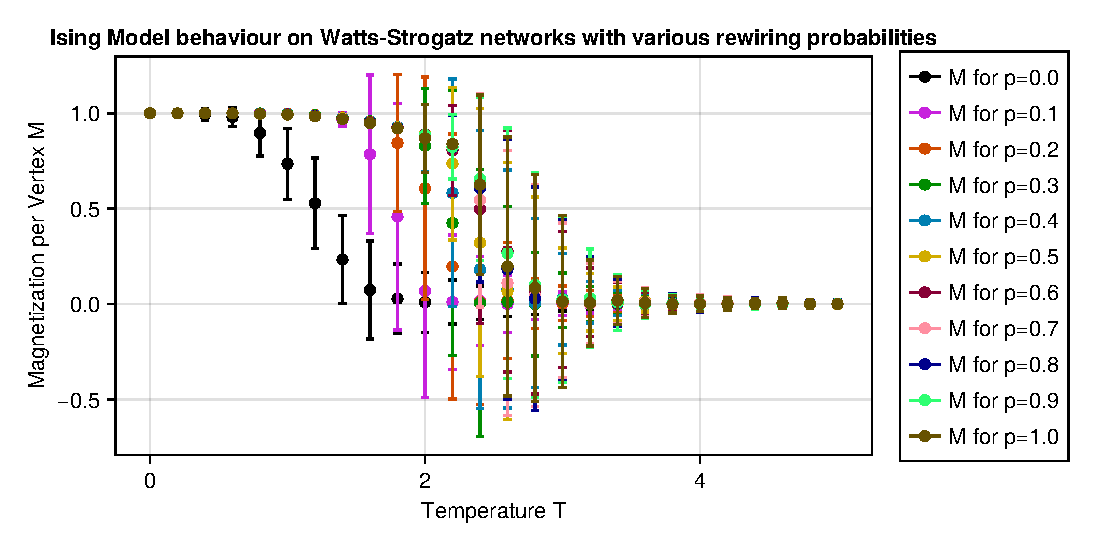
\includegraphics{Ising_magnetization_WS_many}
	\caption{Behaviour of the magnetization of an Ising model on-top a Watts-Strogatz graph for a collection of temperatures and rewiring probabilities}
	\label{fig:M-WS-0.1}
\end{figure}

\subsubsection{Stochastic Block Model}
For the stochastic block model a total of 8 communities with intra-community links having a fixed probability of \num{0.05} will be used, while the modified parameter is the ratio of inter to intra is modified between 0 and 1.
\begin{figure}[h]
	\centering
	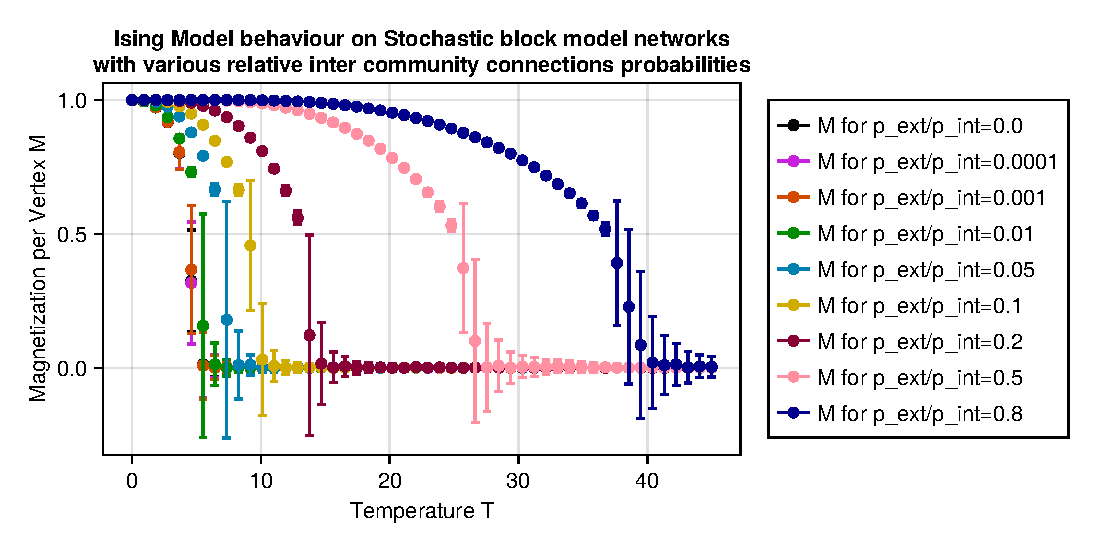
\includegraphics{Ising_magnetization_SBM_many}
	\caption{Behaviour of the magnetization of an Ising model on-top a stochastic block model graph for a collection of temperatures and relative inter-community edge probabilities}
	\label{fig:M-SBM-0.1}
\end{figure}
Here one can again see a strong correlation between the mixing parameter and the temperature at which the magnetization begins to decrease.
A similar argument to the Erdös-Renyi seems plausible, for very low mixing between the communities, they evolve independently and thus different clusters can both be homogeneously magnetized but opposite to other clusters, which in turn lowers total magnetization of the graph.

\newpage